\documentclass[11pt]{article}

\usepackage[margin=1in]{geometry}
\usepackage[T1]{fontenc}
\usepackage{lmodern}
\usepackage{microtype}
\usepackage{amsmath,amssymb,amsthm,mathtools}
\usepackage{mathrsfs}
\usepackage[dvipsnames]{xcolor}
\usepackage[most]{tcolorbox}
\usepackage{tikz}
\usetikzlibrary{decorations.markings,patterns}
\usepackage{enumitem}
\usepackage{tocloft}
\usepackage[hidelinks]{hyperref}

\definecolor{courseblue}{HTML}{1F4E79}
\definecolor{lightblue}{HTML}{EAF2F8}
\definecolor{lightgreen}{HTML}{EAF7EA}
\definecolor{lightpink}{HTML}{FCE8EF}
\definecolor{lightyellow}{HTML}{FFF8D6}
\definecolor{warningyellow}{HTML}{D6A000}
\definecolor{exercisebg}{HTML}{FDEAEA}
\definecolor{exerciseframe}{HTML}{B54040}
\definecolor{examplebg}{HTML}{F4FAFE}
\definecolor{exampleframe}{HTML}{85C1E9}
\definecolor{darkgray}{HTML}{333333}
\definecolor{lightorange}{HTML}{FDEBD8}
\definecolor{orangeframe}{HTML}{E08A3C}

\setlength{\parindent}{0pt}
\setlength{\parskip}{0.65em}
\setlist[itemize]{topsep=0.25em,itemsep=0.15em}
\renewcommand{\cftsecleader}{\cftdotfill{\cftdotsep}}
\renewcommand{\cftsubsecleader}{\cftdotfill{\cftdotsep}}

\theoremstyle{plain}
\newtheorem{theorem}{Theorem}[section]
\newtheorem{proposition}[theorem]{Proposition}
\newtheorem{lemma}[theorem]{Lemma}
\newtheorem{corollary}[theorem]{Corollary}
\theoremstyle{definition}
\newtheorem{definition}[theorem]{Definition}
\newtheorem{example}[theorem]{Example}
\newtheorem{exercise}[theorem]{Exercise}
\theoremstyle{remark}
\newtheorem*{remark}{Remark}
\newtheorem*{fact}{Fact}
\newtheorem*{warning}{Warning}

\tcolorboxenvironment{definition}{
  enhanced,
  unbreakable,
  colback=lightgreen,
  colframe=ForestGreen,
  boxrule=0.7pt,
  arc=2pt,
  left=6pt,
  right=6pt,
  top=5pt,
  bottom=5pt
}

\tcolorboxenvironment{warning}{
  enhanced,
  colback=lightyellow,
  colframe=warningyellow,
  boxrule=0.7pt,
  arc=2pt,
  left=6pt,
  right=6pt,
  top=5pt,
  bottom=5pt
}

\tcolorboxenvironment{exercise}{
  enhanced,
  colback=exercisebg,
  colframe=exerciseframe,
  boxrule=1pt,
  arc=2pt,
  left=6pt,
  right=6pt,
  top=5pt,
  bottom=5pt
}

\tcolorboxenvironment{example}{
  enhanced,
  colback=examplebg,
  colframe=exampleframe,
  boxrule=0.7pt,
  arc=2pt,
  left=6pt,
  right=6pt,
  top=5pt,
  bottom=5pt
}

\numberwithin{equation}{section}

\newcommand{\be}{\begin{eqnarray}}
\newcommand{\ee}{\end{eqnarray}}
\newcommand{\C}{\mathbb{C}}
\newcommand{\R}{\mathbb{R}}
\newcommand{\N}{\mathbb{N}}
\newcommand{\Z}{\mathbb{Z}}
\DeclareMathOperator{\Log}{Log}
\DeclareMathOperator{\Arg}{Arg}

\DeclareMathOperator{\Hol}{\mathcal{H}\mathrm{ol}}
\DeclareMathOperator{\Real}{Re}
\DeclareMathOperator{\Imag}{Im}
\newcommand{\A}{\mathcal{A}}
\newcommand{\CT}{\C[[T]]}
\newcommand{\CLT}{\C((T))}
\tcbset{breakable}
\begin{document}

\begin{center}
  \colorbox{lightblue}{%
    \begin{minipage}{0.94\textwidth}
      \vspace{0.55em}
      \begin{tabular*}{\textwidth}{@{\extracolsep{\fill}}lr}
        {\color{courseblue}\bfseries\LARGE Lecture 19} &
        {\color{courseblue}\bfseries\LARGE MATH 411}\\[0.35em]
        \textbf{Fall 2026} & \textbf{Date: Oct 23, 2026}\\
        & \textbf{Instructor: Manish Patnaik}
      \end{tabular*}
      \vspace{0.45em}
    \end{minipage}}
\end{center}

\setcounter{tocdepth}{1}
\tableofcontents
\vspace{0.45em}


% Sources: Section 6 of the former Lecture 18 (handwritten Lecture 18,
% Oct. 24, pages 7--10), followed by handwritten Lecture 19, Oct. 26,
% pages 1--6. Preserve the handwritten order: logarithm laws, local
% logarithm series, analyticity theorem, Liouville, then the theorem's proof.
% Correct the sign in the logarithm series and supply uniform convergence
% and the closed-disc hypothesis needed for the contour integrals.
We continue Lecture~18 with logarithms of nonvanishing functions.
We then compare logarithms with their local power series and prove that
\emph{every holomorphic function is analytic}. The same integral formula
for the coefficients gives Cauchy's estimates and Liouville's theorem.

\section{Logarithms of nonvanishing analytic functions}
% Handwritten Lecture 18, pages 7--10. Retain the handwritten correction
% from "holomorphic" to "analytic" so f'/f is known to be holomorphic
% before the later theorem that all holomorphic functions are analytic.
The same construction works for a nonvanishing function $f$, replacing
$1/z$ by its \emph{logarithmic derivative} $f'/f$.
As in the handwritten notes, we assume here that $f$ is \emph{analytic}.
Then $f'$ is analytic, so $f'/f$ is holomorphic when $f$ has no zeros.
This uses only facts about power series already established in the course.

\begin{theorem}\label{thm:log-f}
Let $U\subseteq\C$ be simply connected, and let $f$ be analytic on $U$
with $f(z)\ne0$ for all $z\in U$. Choose $z_0\in U$ and $w_0\in\C$
satisfying $e^{w_0}=f(z_0)$. Then
\[
 \boxed{\displaystyle L_f(z)=w_0+
 \int_{z_0}^z\frac{f'(\zeta)}{f(\zeta)}\,d\zeta}
\]
is holomorphic on $U$, satisfies $L_f(z_0)=w_0$, and has the properties
\[
 L_f'(z)=\frac{f'(z)}{f(z)},\qquad e^{L_f(z)}=f(z).
\]
Thus $L_f$ is a holomorphic logarithm of $f$ on $U$.
\end{theorem}
\begin{proof}
The primitive theorem from Lecture~18 applies to $f'/f$, so the integral is
path independent and gives the asserted derivative. Compute
\begin{align*}
 \frac{d}{dz}\bigl(e^{-L_f(z)}f(z)\bigr)
 &=-L_f'(z)e^{-L_f(z)}f(z)+e^{-L_f(z)}f'(z)\\
 &=e^{-L_f(z)}\left[-\frac{f'(z)}{f(z)}f(z)+f'(z)\right]=0.
\end{align*}
Since $U$ is connected, $e^{-L_f(z)}f(z)$ is constant. Evaluating at
$z_0$ gives $e^{-w_0}f(z_0)=1$. Hence $e^{L_f(z)}=f(z)$.
\end{proof}


\begin{center}
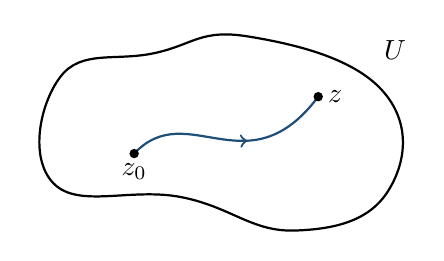
\begin{tikzpicture}[scale=0.85]
 \draw[thick] plot[smooth cycle,tension=0.75] coordinates
 {(-2.6,-0.6) (-2.5,1) (-1.1,1.35) (0.3,1.6) (2.3,0.8)
  (2.4,-0.7) (1,-1.3) (-0.7,-0.8)};
 \node at (2.5,1.4) {$U$};
 \draw[courseblue,thick,postaction={decorate},
 decoration={markings,mark=at position 0.58 with {\arrow{>}}}]
 (-1.4,-0.15) .. controls (-0.6,0.7) and (0.3,-0.7) .. (1.35,0.7);
 \fill (-1.4,-0.15) circle(2pt) node[below] {$z_0$};
 \fill (1.35,0.7) circle(2pt) node[right] {$z$};
\end{tikzpicture}

{\small Integrate $f'/f$ along any path in the simply connected domain $U$.}
\end{center}

\subsection{Dependence on the choices}
\begin{proposition}[Uniqueness up to $2\pi i\Z$]\label{prop:log-unique}
Let $U$ be connected and open. If $L_f$ and $\widetilde L_f$ are two
holomorphic logarithms of the same nonvanishing function $f$ on $U$, then
\[
 \widetilde L_f(z)-L_f(z)=2\pi i k\qquad(z\in U)
\]
for one fixed integer $k$. In particular, prescribing the value at one
point determines the logarithm uniquely.
\end{proposition}
\begin{proof}
Differentiating $e^{L_f}=e^{\widetilde L_f}=f$ shows that both derivatives
are $f'/f$. Their difference has derivative zero, so it is a constant
$C$ on $U$. Since $e^C=1$, we have $C=2\pi i k$ for some $k\in\Z$.
\end{proof}
If we change the starting point from $z_0$ to $z_1$ and choose the new
initial value to be $L_f(z_1)$, we recover exactly the same function:
\[
 L_f(z_1)+\int_{z_1}^z\frac{f'(\zeta)}{f(\zeta)}\,d\zeta=L_f(z).
\]
Choosing another allowed initial value changes the entire logarithm by
one constant multiple of $2\pi i$.

\begin{example}[Different branches on the same slit plane]
For $f(z)=z$ on $U_0=\C\setminus(-\infty,0]$, take $z_0=1$.
The choice $w_0=0$ gives $\Log z=\ln r+i\theta$, with
$-\pi<\theta<\pi$. The choice $w_0=2\pi i$ gives
\[
 L(z)=\Log z+2\pi i=\ln r+i\theta+2\pi i.
\]
Both exponentiate to $z$, and both have derivative $1/z$.
\end{example}

\begin{exercise}
Let $f$ be a nonvanishing analytic function on a simply connected domain
$U$, and let $n\geq2$ be an integer. Use a holomorphic logarithm $L_f$
to construct a holomorphic function $g$ on $U$ such that $g^n=f$.
How does changing $L_f$ by $2\pi i k$ change the root $g$?
\end{exercise}

\section{Logarithms and products}
% Handwritten Lecture 19, pages 1--2.
Do logarithms satisfy the familiar rule
$L_{f_1f_2}=L_{f_1}+L_{f_2}$? The answer depends on the initial values.
Let $f_1,f_2$ be nonvanishing analytic functions on the same simply
connected domain $U$, and fix $z_0\in U$. Choose
\[
 e^{w_1}=f_1(z_0),\qquad e^{w_2}=f_2(z_0),\qquad
 e^{w_{12}}=f_1(z_0)f_2(z_0).
\]
The corresponding integral constructions give
\begin{align*}
 L_{f_1f_2}(z)
 &=w_{12}+\int_{z_0}^z\frac{(f_1f_2)'(\zeta)}{f_1(\zeta)f_2(\zeta)}\,d\zeta\\
 &=w_{12}+\int_{z_0}^z\left(\frac{f_1'(\zeta)}{f_1(\zeta)}
                     +\frac{f_2'(\zeta)}{f_2(\zeta)}\right)\,d\zeta\\
 &=L_{f_1}(z)+L_{f_2}(z)+(w_{12}-w_1-w_2).
\end{align*}
Thus the product rule holds exactly if we choose
$w_{12}=w_1+w_2$. This is always an allowed choice, since
$e^{w_1+w_2}=f_1(z_0)f_2(z_0)$. For independently chosen branches,
$w_{12}-w_1-w_2$ may instead be a nonzero multiple of $2\pi i$.

\begin{example}[The normalized logarithm on the slit plane]
On $U_0=\C\setminus(-\infty,0]$, the choices $f(z)=z$, $z_0=1$,
and $w_0=0$ give the principal logarithm $\Log z$ of Lecture~18.
Its normalization is $\Log 1=0$.
\begin{center}
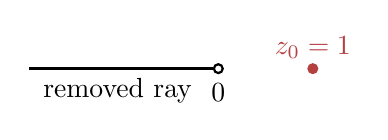
\begin{tikzpicture}[scale=0.8]
 \draw[very thick] (-3,0)--(-0.08,0);
 \draw[fill=white,thick] (0,0) circle(0.07);
 \node[below] at (0,-0.08) {$0$};
 \fill[exerciseframe] (1.5,0) circle(2.5pt) node[above] {$z_0=1$};
 \node[below] at (-1.6,0) {removed ray};
\end{tikzpicture}
\end{center}
Prescribing principal values separately does not guarantee the product
rule: recall the example $z=w=e^{3\pi i/4}$ from Lecture~18.
\end{example}

\section{The logarithm as a local power series}
% Handwritten Lecture 19, pages 2--3.
We know the real logarithm has a power series near $1$. Start directly
with its complex counterpart:
\[
 L_0(1+w):=\sum_{n=1}^{\infty}\frac{(-1)^{n-1}}{n}w^n.
\]
The radius of convergence is $1$, because
$\limsup_{n\to\infty}(1/n)^{1/n}=1$. For $|w|<1$, termwise
differentiation and the geometric series give
\[
 \frac{d}{dw}L_0(1+w)=\sum_{n=1}^{\infty}(-1)^{n-1}w^{n-1}
 =\frac{1}{1+w},\qquad L_0(1)=0.
\]

\subsection{Comparison with the integral construction}
Let $L$ be a holomorphic logarithm of $z$ on a domain
$U\subseteq\C\setminus\{0\}$, and fix $z_0\in U$. Put $w_0=L(z_0)$,
so $e^{w_0}=z_0$. Choose $r>0$ such that
$D(z_0,r)\subseteq U$ and $r<|z_0|$. On this disc define
\begin{align*}
 F(z)&:=w_0+L_0\!\left(1+\frac{z-z_0}{z_0}\right)\\
 &=w_0+\sum_{n=1}^{\infty}\frac{(-1)^{n-1}}{n z_0^n}(z-z_0)^n.
\end{align*}
This is analytic, and
\[
 F(z_0)=w_0,\qquad
 F'(z)=\frac{1}{z_0}\frac{1}{1+(z-z_0)/z_0}=\frac1z.
\]
But $L'(z)=1/z$ as well. Therefore $F-L$ has derivative zero on the
connected disc $D(z_0,r)$ and vanishes at $z_0$. It follows that
\[
 \boxed{\displaystyle
 L(z)=L(z_0)+\sum_{n=1}^{\infty}\frac{(-1)^{n-1}}{n z_0^n}(z-z_0)^n
 \quad (|z-z_0|<r).}
\]
In particular, every holomorphic branch of the logarithm is analytic.
This conclusion uses the explicit power series, before the general
holomorphic-implies-analytic theorem has been proved.

\begin{center}
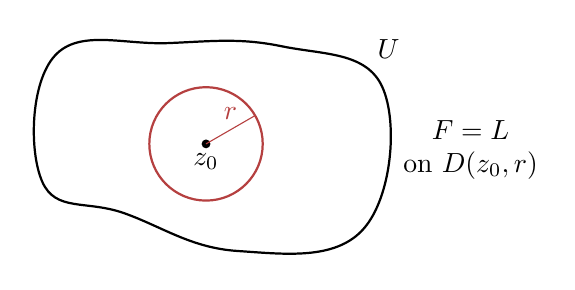
\begin{tikzpicture}[scale=0.8]
 \draw[thick] plot[smooth cycle,tension=0.7] coordinates
 {(-2.8,-0.5) (-2.6,1.5) (-0.8,1.7) (1,1.65) (2.6,1)
  (2.3,-1.25) (0.3,-1.6) (-1.5,-1)};
 \node at (2.7,1.6) {$U$};
 \draw[exerciseframe,thick] (-0.2,0.1) circle(0.9);
 \fill (-0.2,0.1) circle(2pt) node[below] {$z_0$};
 \draw[exerciseframe] (-0.2,0.1)--(0.58,0.55) node[midway,above] {$r$};
 \node[align=center] at (4,0) {$F=L$\\on $D(z_0,r)$};
\end{tikzpicture}
\end{center}

\subsection{The picture of overlapping discs}
The handwritten sketch shows local logarithms on overlapping discs
along a circle around $0$. On each new disc we can adjust the initial
value by a multiple of $2\pi i$ so that the local logarithms agree on
the overlap. Their derivatives are all $1/z$, so matching at one point
makes them agree on the connected overlap.

\begin{center}
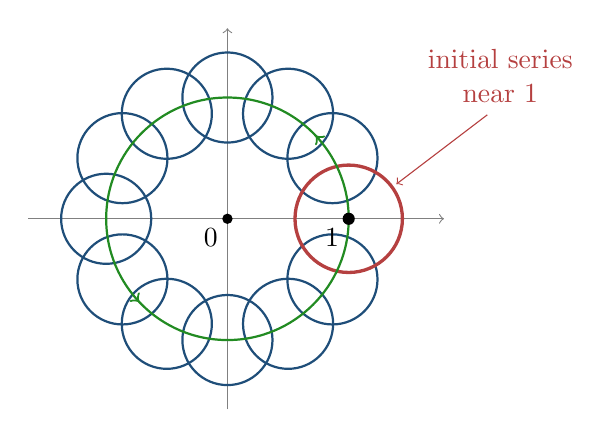
\begin{tikzpicture}[scale=1.1]
 \draw[->,gray] (-2.3,0)--(2.5,0);
 \draw[->,gray] (0,-2.2)--(0,2.2);
 \foreach \a in {30,60,...,330} {
  \draw[courseblue,thick] ({1.4*cos(\a)},{1.4*sin(\a)}) circle(0.52);
 }
 \draw[exerciseframe,very thick] (1.4,0) circle(0.62);
 \draw[ForestGreen,thick,postaction={decorate},
 decoration={markings,mark=at position 0.12 with {\arrow{>}},
 mark=at position 0.62 with {\arrow{>}}}] (1.4,0) arc(0:360:1.4);
 \fill (0,0) circle(1.7pt) node[below left] {$0$};
 \fill (1.4,0) circle(2pt) node[below left] {$1$};
 \draw[exerciseframe,->] (3,1.2)--(1.95,0.4);
 \node[exerciseframe,align=center] at (3.15,1.65)
 {initial series\\near $1$};
\end{tikzpicture}

{\small Local branches can be matched along a path around the origin.}
\end{center}
After one counterclockwise turn, the continued value has increased by
\[
 \int_{|z|=1}\frac{dz}{z}=2\pi i.
\]
Thus local agreement along the path does not give a single-valued
logarithm on all of $\C\setminus\{0\}$. This is the obstruction that
simple connectedness removes in the integral construction.

\section{Holomorphic functions are analytic}
% Handwritten Lecture 19, page 4. State the theorem, give Liouville's
% theorem as in pages 4--5, and then return to the proof on pages 5--6.
The logarithm illustrates a general phenomenon. Cauchy's integral
formula produces a convergent power series for any holomorphic function.

\begin{theorem}[Power series expansion and Cauchy estimates]\label{thm:analytic}
Let $U\subseteq\C$ be open and $f$ holomorphic on $U$. Suppose
$\overline{D(z_0,R)}\subseteq U$, where $R>0$, and let
$\gamma_R(t)=z_0+Re^{it}$, $0\leq t\leq2\pi$, be the positively
oriented boundary circle. Set
\[
 a_n:=\frac{1}{2\pi i}\int_{\gamma_R}
       \frac{f(\zeta)}{(\zeta-z_0)^{n+1}}\,d\zeta
 \quad(n\geq0),\qquad
 M_R:=\max_{\zeta\in\gamma_R}|f(\zeta)|.
\]
Then
\begin{enumerate}
 \item $\displaystyle |a_n|\leq\frac{M_R}{R^n}$ for all $n\geq0$
       \quad\emph{(Cauchy estimates)};
 \item $\displaystyle f(z)=\sum_{n=0}^{\infty}a_n(z-z_0)^n$
       for $|z-z_0|<R$.
\end{enumerate}
The series converges uniformly on each closed disc
$\overline{D(z_0,s)}$ with $0<s<R$. Consequently, $f$ is analytic on $U$.
\end{theorem}

\begin{center}
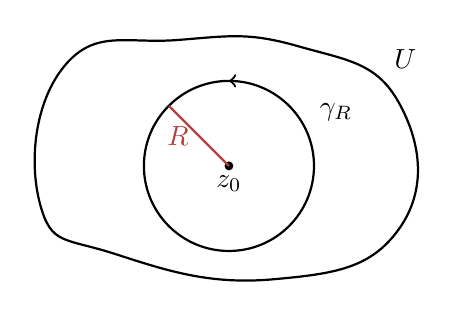
\begin{tikzpicture}[scale=0.8]
 \draw[thick] plot[smooth cycle,tension=0.8] coordinates
 {(-3,-0.6) (-2.6,1.6) (-0.8,2) (1.1,1.9) (2.7,1)
  (2.7,-1) (0.7,-1.8) (-1.8,-1.4)};
 \node at (2.8,1.7) {$U$};
 \draw[thick,postaction={decorate},decoration={markings,
 mark=at position 0.25 with {\arrow{>}}}] (1.35,0) arc(0:360:1.35);
 \fill (0,0) circle(2pt) node[below] {$z_0$};
 \draw[exerciseframe,thick] (0,0)--(-0.95,0.95) node[midway,left] {$R$};
 \node at (1.7,0.85) {$\gamma_R$};
\end{tikzpicture}
\end{center}
The closed-disc condition ensures that $f$ is holomorphic on a
neighborhood of the contour and its interior. For $n=0$, the coefficient
formula is simply Cauchy's formula at the center: $a_0=f(z_0)$.

\subsection{An immediate consequence: Liouville's theorem}
\begin{corollary}[Liouville's theorem]
Every bounded entire function is constant.
\end{corollary}
\begin{proof}[Proof using Theorem~\ref{thm:analytic}]
Suppose $f$ is holomorphic on $\C$ and $|f(z)|\leq M$ for all $z$.
Expand at $z_0=0$. For every $R>0$, the theorem gives
\[
 f(z)=\sum_{n=0}^{\infty}a_n z^n\quad(|z|<R),\qquad
 |a_n|\leq\frac{M}{R^n}.
\]
The coefficients are independent of $R$: power series representing the
same function near $0$ have unique coefficients (equivalently,
$a_n=f^{(n)}(0)/n!$). For each fixed $n\geq1$, let $R\to\infty$.
Then $a_n=0$. Since $R$ can be arbitrarily large, $f(z)=a_0$ on all of $\C$.
\end{proof}
We now prove the expansion theorem used above.

\section{Proof of the power series expansion}
% Handwritten Lecture 19, pages 5--6, with the interchange of sum and
% integral and the final remainder estimate written out.
\begin{proof}[Proof of Theorem~\ref{thm:analytic}]
\textbf{Step 1: estimate the coefficients.}
On $\gamma_R$, we have $|\zeta-z_0|=R$, and the contour has length
$2\pi R$. The estimation lemma gives
\[
 |a_n|\leq\frac{1}{2\pi}\,(2\pi R)\,
              \frac{M_R}{R^{n+1}}=\frac{M_R}{R^n}.
\]

\textbf{Step 2: expand the Cauchy kernel.}
Fix $0<s<R$. For $|z-z_0|\leq s$ and $\zeta\in\gamma_R$,
\[
 \left|\frac{z-z_0}{\zeta-z_0}\right|\leq\frac{s}{R}<1.
\]
Consequently,
\begin{align*}
 \frac{1}{\zeta-z}
 &=\frac{1}{\zeta-z_0}\,
   \frac{1}{1-\dfrac{z-z_0}{\zeta-z_0}}\\
 &=\frac{1}{\zeta-z_0}
    \sum_{n=0}^{\infty}\left(\frac{z-z_0}{\zeta-z_0}\right)^n
 =\sum_{n=0}^{\infty}\frac{(z-z_0)^n}{(\zeta-z_0)^{n+1}}.
\end{align*}
The absolute value of the $n$th term is at most
$R^{-1}(s/R)^n$. Since these bounds form a convergent geometric series,
the kernel series converges uniformly for all such $z$ and $\zeta$.

\begin{center}
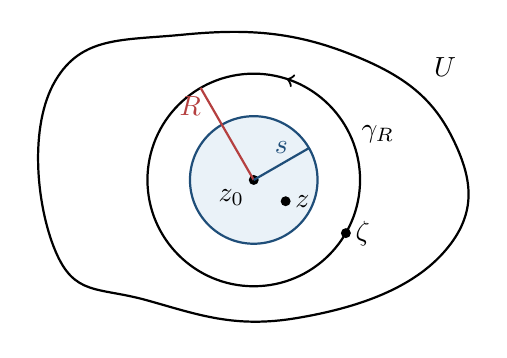
\begin{tikzpicture}[scale=0.9]
 \draw[thick] plot[smooth cycle,tension=0.75] coordinates
 {(-2.8,-1) (-2.8,1.4) (-1,2.05) (1.3,1.8) (2.8,0.6)
  (2.7,-1) (0.6,-1.95) (-1.5,-1.7)};
 \node at (2.7,1.6) {$U$};
 \draw[thick,postaction={decorate},decoration={markings,
 mark=at position 0.2 with {\arrow{>}}}] (1.5,0) arc(0:360:1.5);
 \draw[courseblue,thick,fill=lightblue] (0,0) circle(0.9);
 \fill (0,0) circle(2pt) node[below left] {$z_0$};
 \draw[exerciseframe,thick] (0,0)--(-0.75,1.3)
 node[pos=0.8,left] {$R$};
 \draw[courseblue,thick] (0,0)--(0.78,0.45) node[midway,above] {$s$};
 \fill (0.45,-0.3) circle(2pt) node[right] {$z$};
 \fill (1.3,-0.75) circle(2pt) node[right] {$\zeta$};
 \node at (1.75,0.65) {$\gamma_R$};
\end{tikzpicture}

{\small The smaller disc gives a uniform ratio $s/R<1$ on the contour.}
\end{center}

\textbf{Step 3: integrate term by term.}
Cauchy's integral formula, recalled in Lecture~18, says
\[
 f(z)=\frac{1}{2\pi i}\int_{\gamma_R}\frac{f(\zeta)}{\zeta-z}\,d\zeta
 \qquad (|z-z_0|<R).
\]
The function $f$ is bounded on $\gamma_R$. Multiplying the uniformly
convergent kernel series by $f(\zeta)$ therefore preserves uniform
convergence, allowing termwise integration:
\begin{align*}
 f(z)
 &=\frac{1}{2\pi i}\int_{\gamma_R}
   \sum_{n=0}^{\infty}\frac{f(\zeta)(z-z_0)^n}{(\zeta-z_0)^{n+1}}\,d\zeta\\
 &=\sum_{n=0}^{\infty}\left(\frac{1}{2\pi i}\int_{\gamma_R}
   \frac{f(\zeta)}{(\zeta-z_0)^{n+1}}\,d\zeta\right)(z-z_0)^n\\
 &=\sum_{n=0}^{\infty}a_n(z-z_0)^n.
\end{align*}
More explicitly, the integrated geometric-series remainder satisfies
\[
 \sup_{|z-z_0|\leq s}
 \left|f(z)-\sum_{n=0}^{N}a_n(z-z_0)^n\right|
 \leq M_R\,\frac{(s/R)^{N+1}}{1-s/R}\longrightarrow0.
\]
This also proves uniform convergence on the smaller closed disc.
Every point of $D(z_0,R)$ lies in such a disc, so the expansion holds
throughout $D(z_0,R)$. Finally, every $z_0\in U$ admits some $R>0$
with $\overline{D(z_0,R)}\subseteq U$. Thus $f$ is analytic on $U$.
\end{proof}

\begin{remark}
We already knew that analytic functions are holomorphic by termwise
differentiation of power series. The theorem proves the converse.
In particular, all derivatives of a holomorphic function are themselves
holomorphic. We may now replace ``analytic'' by ``holomorphic'' in the
logarithm theorem at the beginning of this lecture.
\end{remark}
\end{document}
